\chapter{Design}\label{design}

The design of the application will draw from the above requirements and
the associated use cases to form a final application. There are many
decisions to be made when designing an application, each decision needs to be solved in the best way possible given the conditions and the available solutions and development time.

In this chapter some design problems are listed and a discussion is provided for each on a selection of solutions. Each candidate solution is evaluated and compared to other solutions, and a summary of the chosen approach is given in conclusion.

\section{Structure of the information in the solution}\label{structure-of-the-information-in-the-solution}

The application will store notes and code (files) created by the user, however
there are many different ways to store these files. Here are a few of the
different ways to store this information with some positive and negatives of each approach.

\subsection{List of files}\label{list-of-files}

The application could store the notes as a list of simple files in the system.
Each file would have a name and a collection of other attributes: date created,
date modified. This method is the most simple of solutions discussed here however, it does rely on the user to correctly name the files with discipline. If this is done correctly then the list of files solution could be viable.

For example, the following is an idea of how this might look.

\begin{verbatim}
    - Project A - Overview - Project summary
    - Project A - Overview - Change log
    - Project A - Users - User login module
    - Project A - Users - User login module version 2
    - Project B - Overview - Project summary
    - ...
\end{verbatim}
Each line in the above example is a file and each has been named with a logical structure of $ PROJECT - CATEGORY - NAME $

For many reasons this is not an ideal way to view files for a single section of a system. Typically developers work with a single project at once and within that project only a limited subset. This means when the developer has to navigate to a particular file in the system they have to find just one file in what can be a large list.


As a positive consequence of choosing a simple list, the times in which need to
access files across multiple projects. For example in a use case where the developer
needs to switch between projects frequently, the developer can see the
entire list of files without the need to change between folders.

\subsection{Folder structure}\label{folder-structure-i.e.explorer-finder}

There are already existing methods for storing files into folders or
directories. Most mainstream operating systems use a hierarchy of
folders\footnote{Windows has Explorer, and OSX has Finder} to contain files
and more folders. This acts like a tree, each leaf is a file and each subtree
is a folder.

This approach still offers the users free reign over the organization
and naming of each file in the system, however, it also provides the
ability to focus on single parts of the tree at once.

\begin{verbatim}
    - Project A/
      - Overview/
        - Project summary
        - Change log
      - Users/
        - User login module
        - User login module version 2
    - Project B/
      - Overview/
        - Project summary
\end{verbatim}

In the example above the items ending with / are the folders (subtrees) and the
other items are the files (leaf nodes).

This organization into folders can take time to complete and can be done in many
different ways. Within each project, unless managed correctly, there could exist
different ways of creating / naming the folders. This problem of uniformity
crops up in many places within the topic of organization and in general, the
more uniform the structure, the less the user has to remember for each case and
the less brain power needs to be spent understanding it.

There is another problem with a simple tree folder structure, each file in the
folder tree can only exist in one place at once.%
%
\footnote{This can however be solved, as with the unix file system for example.
Symbolic links can allow for files to exist in multiple places at once. }
Some files could be ambiguously belong in multiple places at once. This can make
finding these files take longer. Each ambiguously located file that needs to be
found needs to be searched for in (worst case) all the locations it could be in.

Both the two above problems are lessened by putting sensible limits on
the depth of the folder structure. The reason for this is discussed
below.

\subsection{Simplified folder structure}\label{simplified-folder-structure}

In a simplified folder structure, there are a limited number of levels that can
exist. If viewed as a tree it would have limited depth and contains leaf nodes
(here notes) at the bottom level of the tree.

This simplified structure can help make the choice of folders at each
level more apparent for the user. They have limited choice of
where to place folders and files and as such, the ambiguity problems of a
full folder structure are lessened.

This technique also implicitly limits the user to a set number of
levels. This, although limiting, reduces the number of cases where files have
 more than one obvious location.

\subsection{Tagged files}\label{tagged-files}

In a tagged file organizational system, files are not placed in folders
but instead have each an associated set of ``tags''. Each of these tags
has a name and can be applied to many files.

For example, you might have the following set of files and their tags:

\begin{verbatim}
    - Project summary {Project A, overview}
    - User login module {Project A, Users}
    - Overview {Project A, overview}
    - Project summary {Project B, overview}
\end{verbatim}

The user can then find subsets of files they are interested in by
filtering for the items that have the tags specified:

\begin{verbatim}
    Filter: file has all {Project A, overview}
    Result:
    - Project summary {Project A, overview}
    - Overview {Project A, overview}

    Filter: file has overview
    Result:
    - Project summary {Project A, overview}
    - Overview {Project A, overview}
    - Project summary {Project B, overview}
\end{verbatim}

nb. the folder structure as discussed above
\ref{folder-structure-i.e.explorer-finder} can be represented with a tagged list
of files. This can be achieved by adding a single tag to each file with the path
of the folder that contains it. However the tagging system allows for more
flexibility by allowing multiple tags to exist on the same file.

For some applications, a tagged file system can be both faster and more simple
to understand for the users\cite{ASI:ASI22906}

\subsection{Choice of file organization}\label{choice-of-file-organization}

The simplified folder structure was chosen because of the balance
between the flexible organization of the tagging system and the
simplistic file list. The simplified folder structure proved to be
simple to implement and provides the required functionality.


\begin{figure}
\begin{subfigure}{.5\textwidth}
  \centering
  
\includegraphics[width=.8\linewidth]{Figures/BinderEmpty.png}
  \caption{}
  \label{fig:binderempty}
\end{subfigure}%
\begin{subfigure}{.5\textwidth}
  \centering
  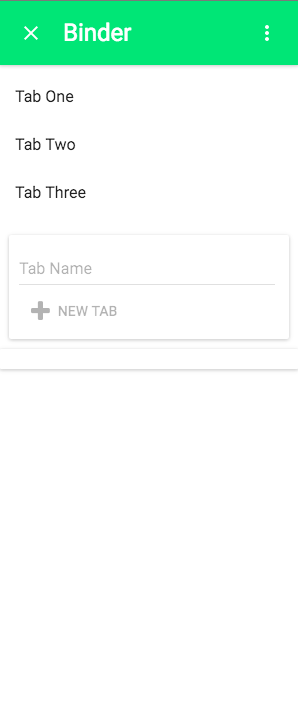
\includegraphics[width=.8\linewidth]{Figures/BinderFull.png}
  \caption{}
  \label{fig:binderfull}
\end{subfigure}
\caption{Binder, top level container for tabs. fig \ref{fig:binderempty} and \ref{fig:binderfull} show empty and full binders respectively}
\label{fig:binder}
\end{figure}

\begin{figure}
\begin{subfigure}{.5\textwidth}
  \centering
  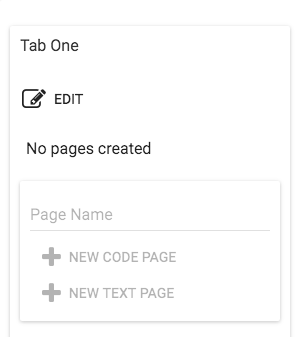
\includegraphics[width=.8\linewidth]{Figures/PagesEmpty.png}
  \caption{}
  \label{fig:pagesempty}
\end{subfigure}%
\begin{subfigure}{.5\textwidth}
  \centering
  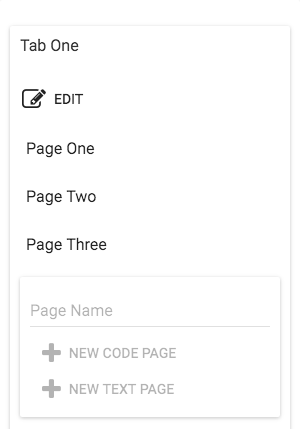
\includegraphics[width=.8\linewidth]{Figures/PagesFull.png}
  \caption{}
  \label{fig:pagesfull}
\end{subfigure}
\caption{Tabs, the second level container. fig \ref{fig:pagesempty} and
\ref{fig:pagesfull} show an empty and full tab respectively. This is shown
when a tab is selected, the pages are listed with the ability to edit the list,
and add new items.}
\label{fig:pages}
\end{figure}

Fig \ref{fig:binder} shows the implemented simple folder structure. The names
given to the levels are as follows: Binder, top level container. Tab, second
level container. Fig \ref{fig:pages} shows how the second level container is
displayed.

\section{Search capability in the system}\label{search-capability-in-the-system}

The requirements gathering process clearly identified in multiple places the
need for the system to provide a quick and simple search function.

There are multiple ways to provide search functionality within a document
management system, some of which are suitable for the application and some are
not. The below is a summary of a few of the options and an evaluation of each.

The search feature should take the users query and provide access to the
matching files in the system. This part of the searching experience will be the
same for all the discussed methods. However the parts that differ in the
compared methods are:
\begin{itemize}
  \item the format of the users query
  \item the searching method
  \item the time taken to perform the search
  \item the presentation of the results
\end{itemize}

\subsection{Simple text search / serial scanning}%
\label{simple-text-search-serial-scanning}

The simplest method for searching in a collection of documents is taking a
simple query from the user (the search term), and searches for the occurrences
of the term in each file. Each match results in an item in the result list
displaying the name of the file, and the position within the document.

For example:

\begin{alltt}
    search term: \emph{test}
    results:
    - File A, line 13, chars 34-38
      - ... the users will then report on \emph{test}ing ...
    - File A, line 13, chars 10-13
      - Chapter 2: \emph{Test}ing ...
\end{alltt}

This technique is simple and for small amounts of files and content is fast to
compute. However, due to the fact that the algorithm is loosely linear in the
number of files this technique would be impractical for large numbers of files.
This technique, called ``serial scanning''\footnote{%
\url{https://en.wikipedia.org/wiki/Full_text_search\#Indexing}%
has more details on this.}%
, is only typically used for smaller amounts of text due to this problem.

\blockquote{ However, when the number of documents to search is potentially
large, or the quantity of search queries to perform is substantial, the problem
of full-text search is often divided into two tasks: indexing and searching.
}\cite{wiki:full-text-search}

This technique that wikipedia refers to is discussed below.

\subsection{Full text index}\label{full-text-index}

When the simple method of searching through all the files becomes too slow, one
alternative is to create a concordance
\footnote{\url{https://en.wikipedia.org/wiki/Concordance_(publishing)} for more
information}. This is a table of words in a publication (here a note) and where
those words appear within the document. By using this concordance in place of
searching the text directly, the application is able to search a smaller amount
of data to find the results and hence speed up the search process.

This requires that there is a pre-processing step before a search can be
completed. This needs to be recalculated each time a user changes a
document so that all subsequent queries can find the new content.

This is the tradeoff with the more complex methods for searching. This method
requires the index to be built / rebuilt before any searching can take place.
However this can be done ``offline'' and cached for later use.

\subsection{Extraction of keywords}\label{extraction-of-keywords}

Another method of searching the documents is by analysis of keywords. Indexing a
select few words per note instead of all the words as in \ref{full-text-index}
means smaller indexes and faster searches.
Either a list of keywords is created and left static or, machine learning
algorithms can learn which words are important within the page and index only
those words.

This is however only applicable when the user's search terms can be limited as
such. This is because if the user searches for a word that is contained within a
file in the application, it will only be found if the word is in the keywords
list. In the case of a note taking application, a search method that can fail to
find a word that exists in the  document is of little use. However indexes of
the popular search terms can help to find preliminary results for a query, or
provide caches of common queries.


%\subsection{Edit distance}\label{edit-distance}

%\begin{quote}
%JP maybe discuss fuzzy search
%\end{quote}

\subsection{Reasons for selecting simple text
search}\label{reasons-for-selecting-simple-text-search}

The numerous ways to search the text within a collection of documents
each provide there own ways to provide the results. While many of the
different search methods are concerned with the performance of a search
and their accuracy in terms of the results, the most basic search
discussed the Simple text search \emph{link above section} as discussed
can offer the features needed by most users of the application.

There are many other features that can be added to the functionality
provided by the Simple text search \emph{link} however these can be
added as an extension to the program after the initial release.

\section{Type of user interface}\label{type-of-user-interface}

The different types of user interface that designers can choose from
when designing applications can be categorized into a few main
categories:

\begin{verbatim}
- Command line
- GUI / WIMPS
\end{verbatim}

For visualizing text, popular command line applications for editing text
like Vim or Emacs do exist however, the richer environment of a GUI
application is predominately preferred with its ability to customize
fonts and other such attributes of the layout and style. They also
provide a better experience for users with the use of menus etc. These
can provide a more simple to use application than an alternate command
line program with many shortcuts to memorize.

There are many different types of GUI application that can be built and
an important decision that needs to be made before selecting the layout
of the application is what platform to build the application on.

\subsection{Native solution for operating
system}\label{native-solution-for-operating-system}

The first platform option is developing a desktop first application
native in a selected operating system. This would require selecting one
of the native windowing API's for the operating system. Some of these
API's are cross platform enabled for example see
\href{http://www.qt.io/}{qt} for a popular choice. Some more polished
and more integrated with the selected operating system for example
Apple's own windowing API is
\href{https://en.wikipedia.org/wiki/Cocoa_(API)}{Cocoa}

The advantages of using the operating system's manufacturer built API is
one of support from the company and choice of open source vs
proprietary. As one of the requirements is that the system should be
accessible the proprietary method is not an option for a time
constrained development like this. In order to complete a cross platform
version using operating system specific (non cross platform) API's would
mean a rewrite of the GUI code for each operating system that was to be
supported. The advantages of using the operating system's manufacturer
built API is one of support from the company and choice of open source
vs proprietary. As one of the requirements is that the system should be
accessible the proprietary method is not an option for a time
constrained development like this. In order to complete a cross platform
version using operating system specific (non cross platform) API's would
mean a rewrite of the GUI code for each operating system that was to be
supported.

\subsection{Mobile solution for Android /
IOS}\label{mobile-solution-for-android-ios}

The production of a mobile application for either the Android or IOS
markets would be done with either two versions of the application as
discussed with the desktop versions above, or there are tools like
\href{https://www.xamarin.com/platform}{Xamarin}

\begin{verbatim}
"Deliver native Android, iOS, and Windows apps, using existing skills,
teams, and code."
*cite xamerin*
\end{verbatim}

This allows for applications to be built for a variety of mobile
platforms with a single code base in C\#. The ability to ``write once
run anywhere'' is a big selling point for Xamarin and others like it.
However it would still restrict users into using mobile only.

\subsection{Browser based solution}\label{browser-based-solution}

With modern advances in browser technology it has become more feasible
to create full desktop replacement applications as website-applications.
These websites are truly cross platform, they can be viewed on any
platform with access to a web browser. Desktop OS or mobile OS alike can
all use one of a multitude of recent browsers from many vendors. -
Chrome (Windows, Mac OSX, IOS, Android) - Safari (Mac OSX, IOS, Windows)
- Opera (Windows, Mac OSX, IOS \{opera-mini\}, Android \{opera-mini\}) -
Firefox (Windows, Mac OSX, IOS, Android)

There are many different libraries on offer to help develop applications
with javascript. However it is still possible to create more traditional
client-server applications and have just a simple lightweight javascript
free front end. These applications tend to be slower and more cumbersome
to use because of there need to communicate every action with a server
over http.

An alternative to the more traditional client-server architecture is the
now more popular single page javascript application. This merges the
lines between the user perceived differences of the desktop and browser
experience.

A single page javascript application is a single web page that functions
like a normal application. The application have all the features of a
desktop application, they can make use of windows, buttons, and
animations etc\ldots{}

External data is gathered in background http calls (called Ajax
requests) and does not necessitate a full page reload. The absence of
these full reloads and the flash of white as the page loads give the
user a much better experience.

\emph{cite}

Single Page Web Applications By Michael S. Mikowski and Josh C. Powell

\subsection{Reason for selecting
browser}\label{reason-for-selecting-browser}

For the application being built the choice of platform is between a
cross platform library for a native desktop application and a web based
solution. For reasons of experience with technology and programming
languages developing for the browser was selected as the platform.

The browser application will be accessible from any platform and device
and provides an easy way to update the application in the future.

There are many different libraries that can help when building a
javascript application in the browser. The libraries have some things in
common and other unique points that set them apart from each other. Most
of the libraries cover the standard principles of MVC ``Model View
Controller'' or some similar variant thereof. See
\href{https://en.wikipedia.org/wiki/List_of_JavaScript_libraries\#Web-application_related_.28MVC.2C_MVVM.29}{here}
for a community populated list on wikipedia.

\subsection{Javascript MVC library -
React.js}\label{javascript-mvc-library---react.js}

React.js is a fairly new open source library from facebook.

\begin{verbatim}
A JAVASCRIPT LIBRARY FOR BUILDING USER INTERFACES

*cite React.js website*
https://facebook.github.io/react/
\end{verbatim}

React.js brings the notions of pure functions to the problem of creating
and updating views. In React.js the headache of updating the view when
something happens in the application is handled automatically. This is
accomplished by having the view hierarchy be a result of applying a pure
function of the application state. This has the important consequence of
removing the need for the developer to tell the application how an
action should update the UI. The developer only needs to update the
state and React.js will work out what needs to change by calculating the
difference in the old and new view hierarchies.

\subsection{Future React Native}\label{future-react-native}

React.js has a new related project created by the same team called React
Native. React Native takes the principles of React.js and with slight
tweaks to the code the same code can run as a native application on both
IOS and Android.

This would provide a way to get the application onto mobile devices in a
native environment the users wouldn't even know that the application was
even running in the browser.

\section{Choice of interface - Notebook
metaphor}\label{choice-of-interface---notebook-metaphor}

The interface of any application need to be simple and easy to
understand. the more complicated the interface the more brainpower needs
to be dedicated to using it. The most successful user interfaces provide
simple intuitive ways for uses to do the actions they require.

\begin{verbatim}
Metaphors are the fundamental concepts, terms, and images
by which information is easily recognized, understood, and
remembered.
- Metaphor Design for User Interfaces, Marcus, Aaron
\end{verbatim}

\emph{cite} @inproceedings\{Marcus:1998:MDU:286498.286577, author =
\{Marcus, Aaron\}, title = \{Metaphor Design for User Interfaces\},
booktitle = \{CHI 98 Cconference Summary on Human Factors in Computing
Systems\}, series = \{CHI '98\}, year = \{1998\}, isbn =
\{1-58113-028-7\}, location = \{Los Angeles, California, USA\}, pages =
\{129--130\}, numpages = \{2\}, url =
\{http://doi.acm.org/10.1145/286498.286577\}, doi =
\{10.1145/286498.286577\}, acmid = \{286577\}, publisher = \{ACM\},
address = \{New York, NY, USA\}, keywords = \{Web, consumers, culture,
diversity, graphic design, icons, information design, metaphors,
multi-media, productivity tools, rhetoric, semantics, semi-otics,
symbols, user interfaces, visible language\}, \}

The metaphor chosen for the application is the notebook. A physical
notebook has pages, tabs etc\ldots{} These are easily understood by
anyone who knows what a notebook is. We can extend the notion of a
notebook with concepts from the wider world of books with indexes and
contents pages.

The application will take from this notion of the ``notebook metaphor''
and from there the application interface will be designed.

\emph{notebook image mapped to uml diagram of application}

\section{Detachment of the SQL interface through custom web
API}\label{detachment-of-the-sql-interface-through-custom-web-api}

Selecting the browser poses some specific problems for a SQL IDE. A SQL
IDE needs to have access to the SQL server in order to execute queries
and retrieve results. There is no support in any of the mainstream
browsers for direct integration with a SQL server database, although
they do have limited support \emph{cite web sql} for in browser
databases.

This therefore requires the production of some middleware to connect the
database to the application. The commonly used method for transferring
data in the browser is via a JSON web API. There are many methods for
connecting to a SQL server database however, the Microsoft documentation
\emph{cite} https://msdn.microsoft.com/en-us/library/ms162132.aspx
contains C\#, VB, C++ documentation and libraries for querying the
database. I have experience using the C\# conneciton methods before and
with this in mind the middleware was chosen to be a C\# website
providing a mapping from JSON to the database.

\emph{diagram of connection}
